\chapter{Applications}
\label{C:Applications}

In many areas of computer vision matching local feature points is a key 
component, and matching algorithms have applications in problems such as
scene matching, object recognition, near duplicate detection and 
panorama recognition. To show the practical applications of the proposed 
matching algorithms, \emph{MM} and \emph{MMC}, we use show how they 
improve existing methods in near duplicate detection and panorama 
recognition. These two problems were chosen because they both involve 
matching images that might or might not overlap. These cases requires 
matching algorithms that limit false positives since e.g. returning the 
top $n$ matches for any given image pair would make it hard to 
distinguish adjacent or duplicate images from non-adjacent or dissimilar
image pairs. Near duplicate detection also constraints normal matching 
algorithms from relying on geometric assumptions, since we have very few
guarantees between two potential near duplicates that they should be 
matched using any particular geometric heuristic. In this section, we 
will first see \emph{MMC} applied to panorama recognition and alignment,
and next \emph{MM} and \emph{MMC} applied to near duplicate detection.


\subsection{Panorama Recognition and Alignment}
One of the oldest practical problems approached in computer vision is 
the automatic stitching of several source images into a bigger image, 
such as panoramas and composite satellite photos\footnote{A brief 
overview of the history of image stitching can be found in Szeliski's 
book: Computer Vision: Algorithms and Applications \cite{szeliski2010}}.  
As part of the process of stitching together images, the individual 
images must be aligned and often transformed in perspective. Earlier 
methods relied on minimizing pixel dissimilarities in overlapping images 
while more recent methods have used local feature points to estimate the 
correct image alignment. Using local feature points carry the additional 
advantage that it is feasible to automatically recognize where each 
source image belong in the final panorama.

\begin{figure}[h]
	\begin{subfigure}[t]{0.9\textwidth}
		\centering
        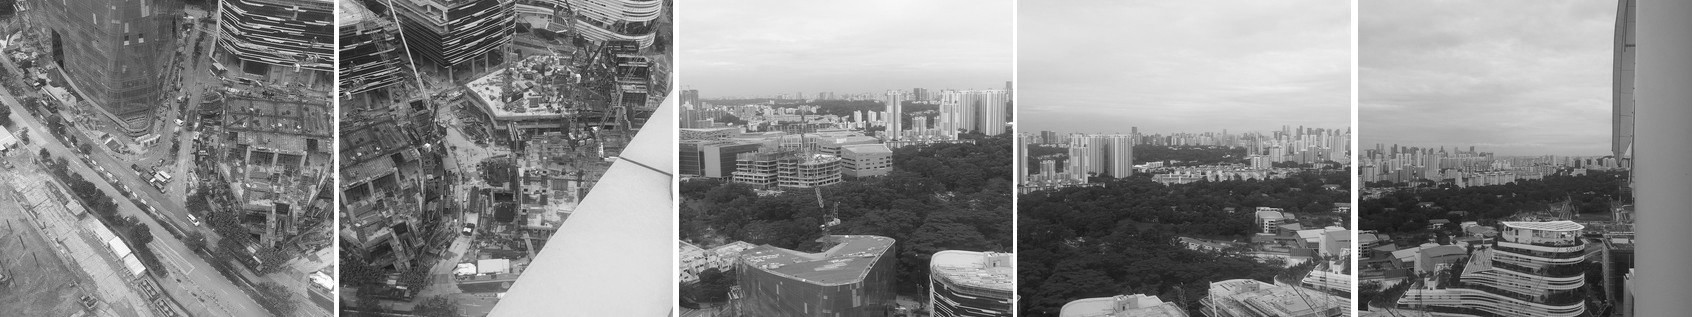
\includegraphics[width=\textwidth]{images/pano_wide}
        \label{fig:pano_images}
		\caption{Source images}
    \end{subfigure}%
	\\
	\centering
    \begin{subfigure}[b]{0.4\textwidth}
		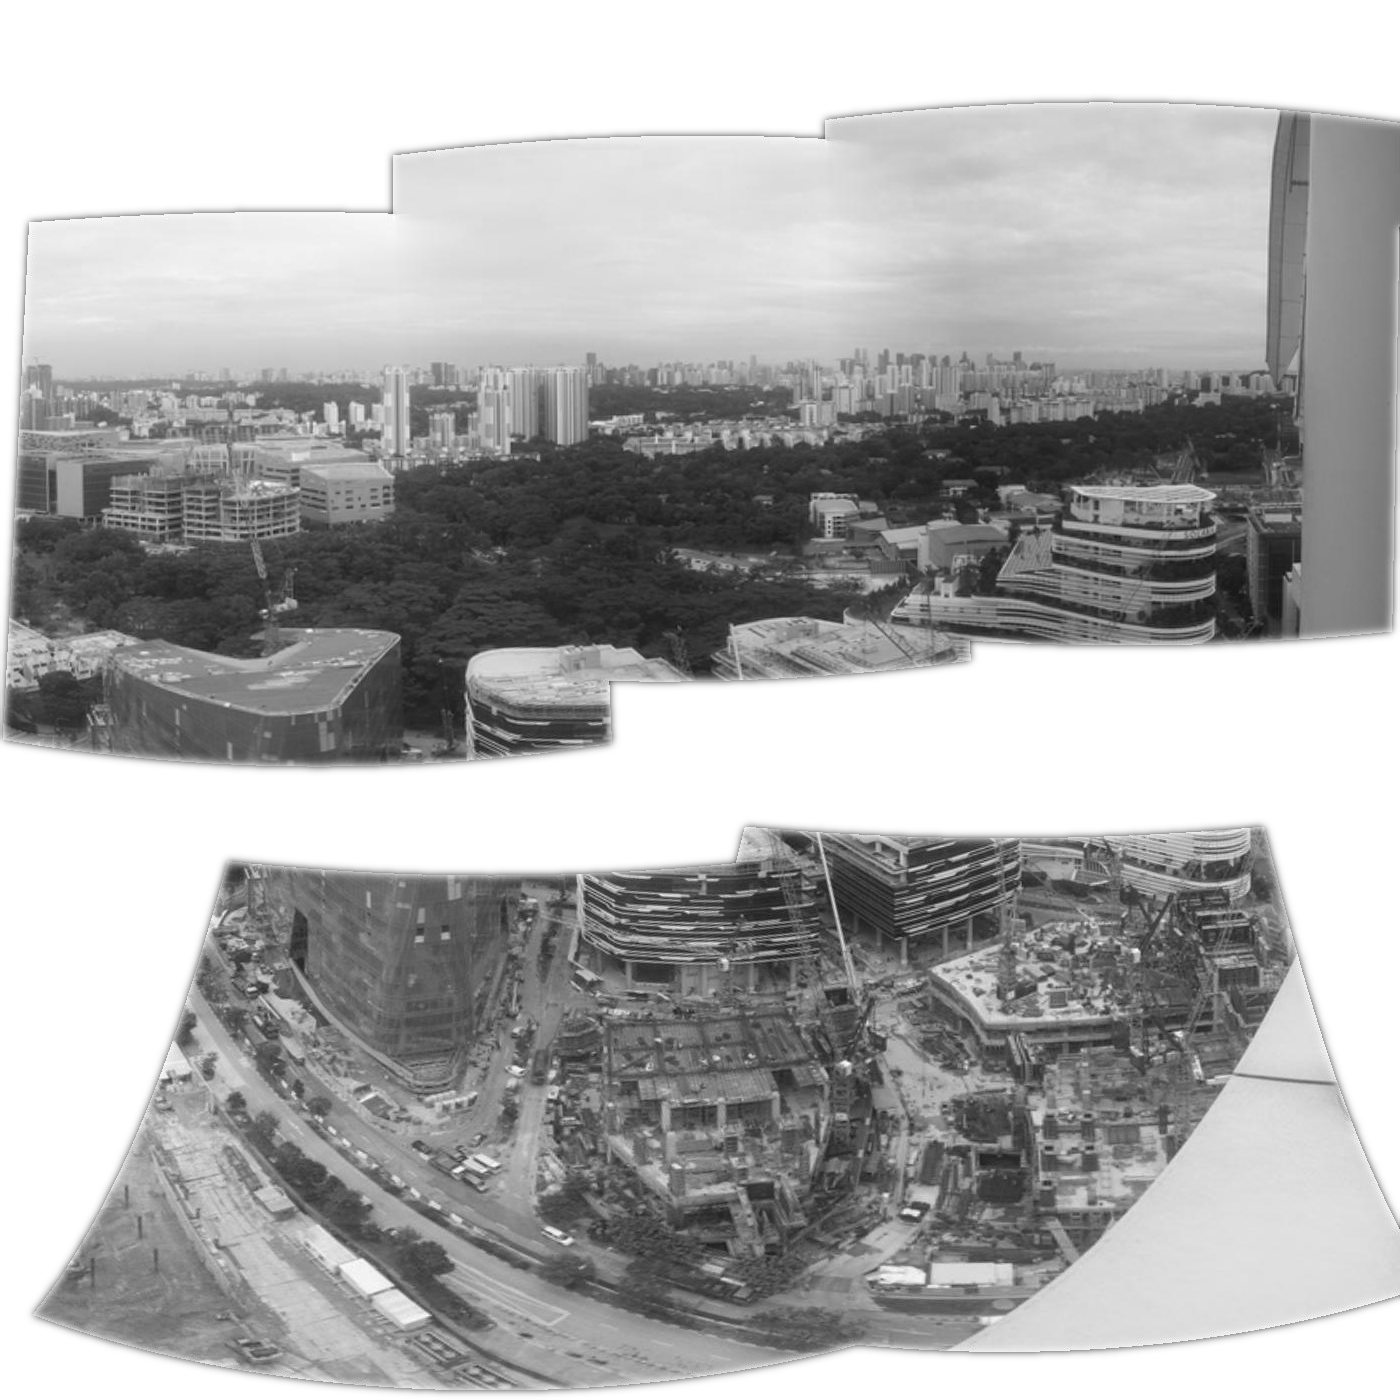
\includegraphics[width=\textwidth]{images/panorama-autostitch}
        \label{fig:pano_autostitch}
		\caption{Panorama by Autostitch}
    \end{subfigure}%
	~%add desired spacing between images, e. g. ~, \quad, \qquad
	%(or a blank line to force the subfigure onto a new line)
    \begin{subfigure}[b]{0.4\textwidth}
		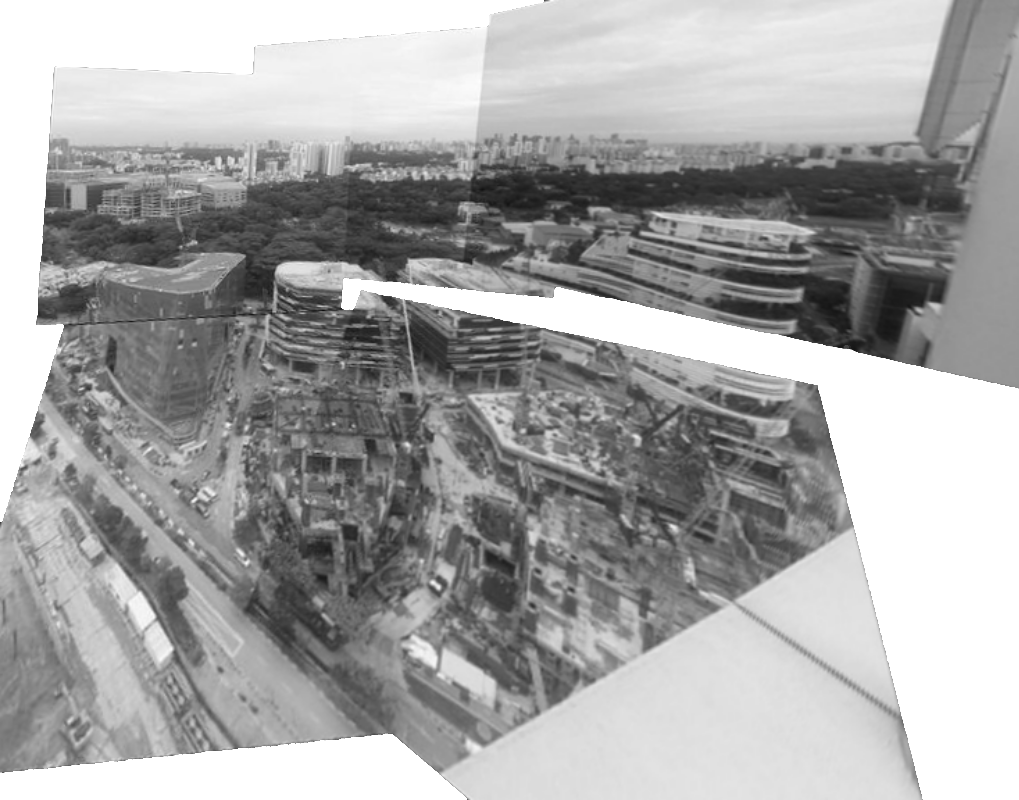
\includegraphics[width=\textwidth]{images/panorama-MMC}
		\caption{Panorama by MMC}
		\label{fig:pano_MMC}
	\end{subfigure}%
    \caption{An example of a difficult case for panorama recognition and 
        alignment.  In a) the source images used to generate the 
        panorama are displayed.\ b) shows the result of the Autostitch 
        program from \cite{brown2007automatic} which fails to combine 
        all images, while c) demonstrates the result of the simple 
        panorama stitcher
	using the proposed MMC algorithm. Here the two left images are 
correctly linked}
    \label{fig:pano_example}
\end{figure}

In \cite{brown2007automatic}, Brown and Lowe demonstrate how a panoramic 
image can be assembled by collecting the feature points of all source 
images and matching them to obtain a set of inter image matches.  By 
using \emph{RANSAC}\footnote{RANdom SAmple Consensus, an iterative 
    algorithm to estimate parameters from noisy data introduced in 
Fischler and Bolles in 1981 \cite{fischler1981ransac}} to find matches 
deemed as inliers between image pairs, they are able to recognize image 
neighbors and align them to construct the final panorama.

This process hinges on the effectiveness of the matching algorithm used 
to match the feature points. Not only is it important that true pairs 
are accurately matched, but since we are matching points in image pairs 
that might not be adjacent in the final panorama, we also need to make 
sure that we consistently reject false positives, i.e.\ proposed matches 
that link feature points which don't correspond.

To demonstrate the usefulness of \emph{MMC} applied to panorama 
recognition and alignment we construct a simple panorama stitcher taking
as input a set of $n$ source images $\left\{I_0, \ldots, I_n\right\}$ 
and returns as output a panoramic image stitched together from the 
source images. Based on the matches found by applying \emph{MMC} to $I$, 
the images are combined in an order corresponding to how many matches 
connect them, as done by Brown and Lowe \cite{brown2007automatic}.

Brown and Lowe make use of bundle adjustment\footnote{Bundle adjustment 
provides a way to globally optimize the accuracy of the image alignment} 
and a lot of image enhancements such as exposure adjustment and edge 
blurring to provide a seamless panorama. While these additions improve 
the end product, they don't influence the performance of panorama 
alignment and recognition and haven't been included in the simple 
comparison algorithm.

Figure~\ref{fig:pano_example} shows an example where the added accuracy 
of MMC enables us to correctly recognitize and align source images that 
fail to be combined by Autostitch, a program using the algorithm 
proposed by Brown and Lowe \cite{brown2007automatic}. In this particular
case the matching algorithm used in Autostitch fails to find sufficient 
matches between two images pairs to correctly position them and 
consequently doesn't produce a panorama containing all images as a 
result.

This example illustrates how an improved matching algorithm can be 
applied to panorama recognition and alignment to allow for panoramas 
created with images that have little overlap.
% Maybe find example of images with identical features that would be 
% hard to match?

\subsection{Near Duplicate Detection}
If we look at two images, we can often easily tell if one image 
resembles the other enough to be redundant in a photo album. In computer 
vision this task becomes a lot less trivial because our idea of a 
duplicate image might only require there being some object or scene in 
common between the image pair. In addition the object or scene might 
have been taken from a different angle and under different camera 
settings. Facing these challenges, a lot of work has been done trying to 
reliably recognize duplicaes both with regards to corporate intellectual 
property as well as consumer photo albums because both applications 
provide useful tools.  A company might be interested in finding images 
that are derived from their intellectual property, while consumers 
taking vacation photos might be interested in grouping duplicate images 
to allow for easier photo organization.

\begin{figure}[h]
	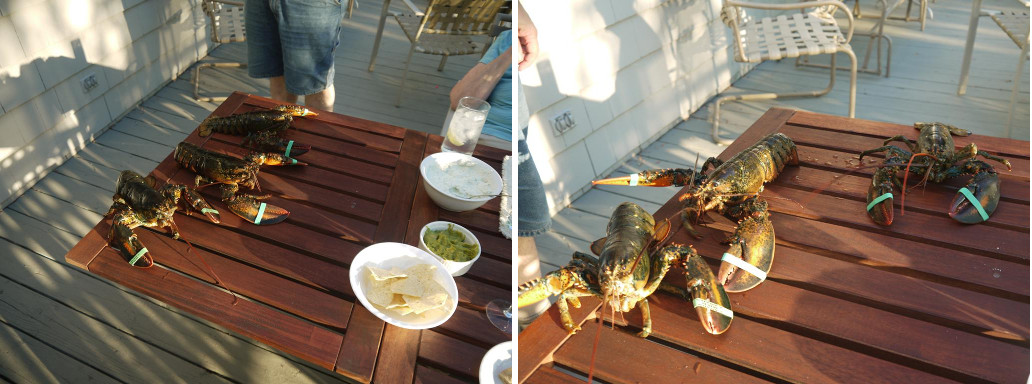
\includegraphics[width=\textwidth]{images/near_duplicate_example}
	\caption{Example of a near duplicate image pair from the 
	California-nd dataset \cite{jinda2012california}}
	\label{fig:near_duplicate}
\end{figure}

Local features are often used to group similar images, either by looking
at a histogram of descriptors \cite{wu2009bundling} or by looking at how
well feature points match between images \cite{zhao2009scale},
\cite{chu2010consumer}, \cite{vas2013cluster}. In the latter case 
finding near duplicates means that we will be matching image pairs that 
might or might not contain any actual matches. In this case we would 
benefit from a reliable matching algorithm that minimizes false 
positives, which is a characteristic of both \emph{MM} and \emph{MMC}.

The \emph{PhotoCluster} method introduced by Vonikakis et al.  
\cite{vas2013cluster} shows the best clustering performance on the 
California-nd dataset \cite{jinda2012california} which contains a set of
annotated vacation images similar to a typical photo album in a consumer
product. \emph{PhotoCluster} works by grouping images in several steps 
using first image metadata and global features to obtain a set of 
proposed clusters. Then local features are used to find the best 
matching images in these proposed clusters yielding the final groups of 
near duplicate images. To show the viability of \emph{MMC} in the 
application of near duplicated detection, we modify the PhotoCluster 
method to use \emph{MMC} for matching images instead of \emph{Ratio} 
which was previously used. Due to the time consumption of \emph{MMC}, 
all images where resized to to 10\% before being compared. Outside of 
that, the experiments were performed exactly as documented in 
\cite{vas2013cluster}.

\begin{table}[htb]
\caption{Results from Near Duplicate Detection at 10\% scale}
\label{table:ndd}
	\centering
%	\small
\begin{tabular}{r*{2}{r}}
\hline
    Method: & Ratio & MMC   \\
	\noalign{\smallskip}
	%
    F1 score: & 0.4654 & 0.5459 \\
	\hline
\end{tabular}
\end{table}

The results of the comparison can be seen in Table~\ref{table:ndd}. It 
shows that \emph{MMC} improves performance by 8.05\% over the original 
framework using \emph{Ratio} to match images. For comparison, the 
performance improvement of \emph{PhotoCluster} compared to XMatch 
\cite{zhao2009scale}, the second best performing algorithm on the 
California-nd dataset according to \cite{vas2013cluster}, is 2.52\%.

